\section{Introduction}

Large Language Models (LLMs) have become indispensable in natural language processing (NLP) \citep{devlin2019bert,brown2020language,kaplan2020scaling,ouyang2022training,wei2022emergent,wei2022chain,touvron2023llama,openai2024gpt4technicalreport}, powering a diverse array of applications such as chatbots \citep{anthropic2023claude,bai2023qwen,openai2024gpt4technicalreport,deepseekai2025deepseekr1incentivizingreasoningcapability}, search engines \citep{google2023bard,microsoft2023bing}, and programming assistants \citep{copilot,claude_3_7} through their capacity to interpret and generate text that mimics human language. These models excel in capturing linguistic nuances, yet their practical deployment is critically dependent on the efficiency of \textit{inference}---the process of generating responses to user queries. This process places significant demands on computational resources, particularly memory and processing capacity, making efficient task scheduling a pressing concern \citep{garcia2019estimation}. The consequences of inefficiency are substantial: inefficient inference not only delays responses (thereby dissatisfies users), but also increases operational costs and environmental footprints \citep{strubell2019energy,desislavov2021compute}. For example, systems such as ChatGPT incur daily inference costs of approximately \$700,000 and consume significant amounts of electricity, leading to considerable carbon emissions \citep{patel2023peeling,patterson2021carbon}. Optimized scheduling provides a means to mitigate these issues by improving users' satisfaction, maximizing resource utilization and reducing ecological impact \citep{wu2022sustainable}.

Understanding the inference process is crucial for addressing its scheduling challenges (refer to Figure \ref{fig:intro_example} for an illustration). When a user submits a query, termed a \textit{prompt} (e.g., ``Is apple a fruit?''), the large language model (LLM) first decomposes it into discrete units called \textit{tokens}, such as [``Is'', ``apple'', ``a'', ``fruit'', ``?'']. These tokens are subsequently transformed into numerical vectors that encode both semantic and positional information. The model then generates a response incrementally, producing one token at a time through an \textit{attention} mechanism \citep{vaswani2017attention}. This mechanism requires maintaining the computational history of all prior tokens to capture dependencies across the sequence, enabling coherent and contextually relevant outputs. To achieve this efficiently, practitioners employ a key-value (KV) cache---a memory structure that stores precomputed attention keys and values for all previously generated tokens. The KV cache is essential because recalculating the attention history for each new token would be computationally prohibitive, significantly slowing down the inference process and rendering it impractical for real-time applications. By caching these key-value pairs, the system avoids redundant computations, thereby accelerating response generation and optimizing resource utilization---a critical consideration in operational settings with high query volumes. For example, as the response to the prompt ``Is apple a fruit?'' develops into ``Yes it is'', the KV cache expands with each word. For the token ``Yes'', the system stores a key-value pair where the key indicates its position (e.g., ``word 1''), and the value encapsulates information about ``Yes'' that facilitates predicting the next token, ``it''. This process continues for each subsequent token, progressively increasing GPU memory consumption. These key-value pairs are critical for determining the sequence of tokens in the response. However, if the KV cache exceeds available memory, the system may encounter performance degradation or failures due to the need to offload data to slower storage mediums \citep{tay2022efficient,kang2024gear,hooper2025kvquant}.
\begin{figure}
    \centering
    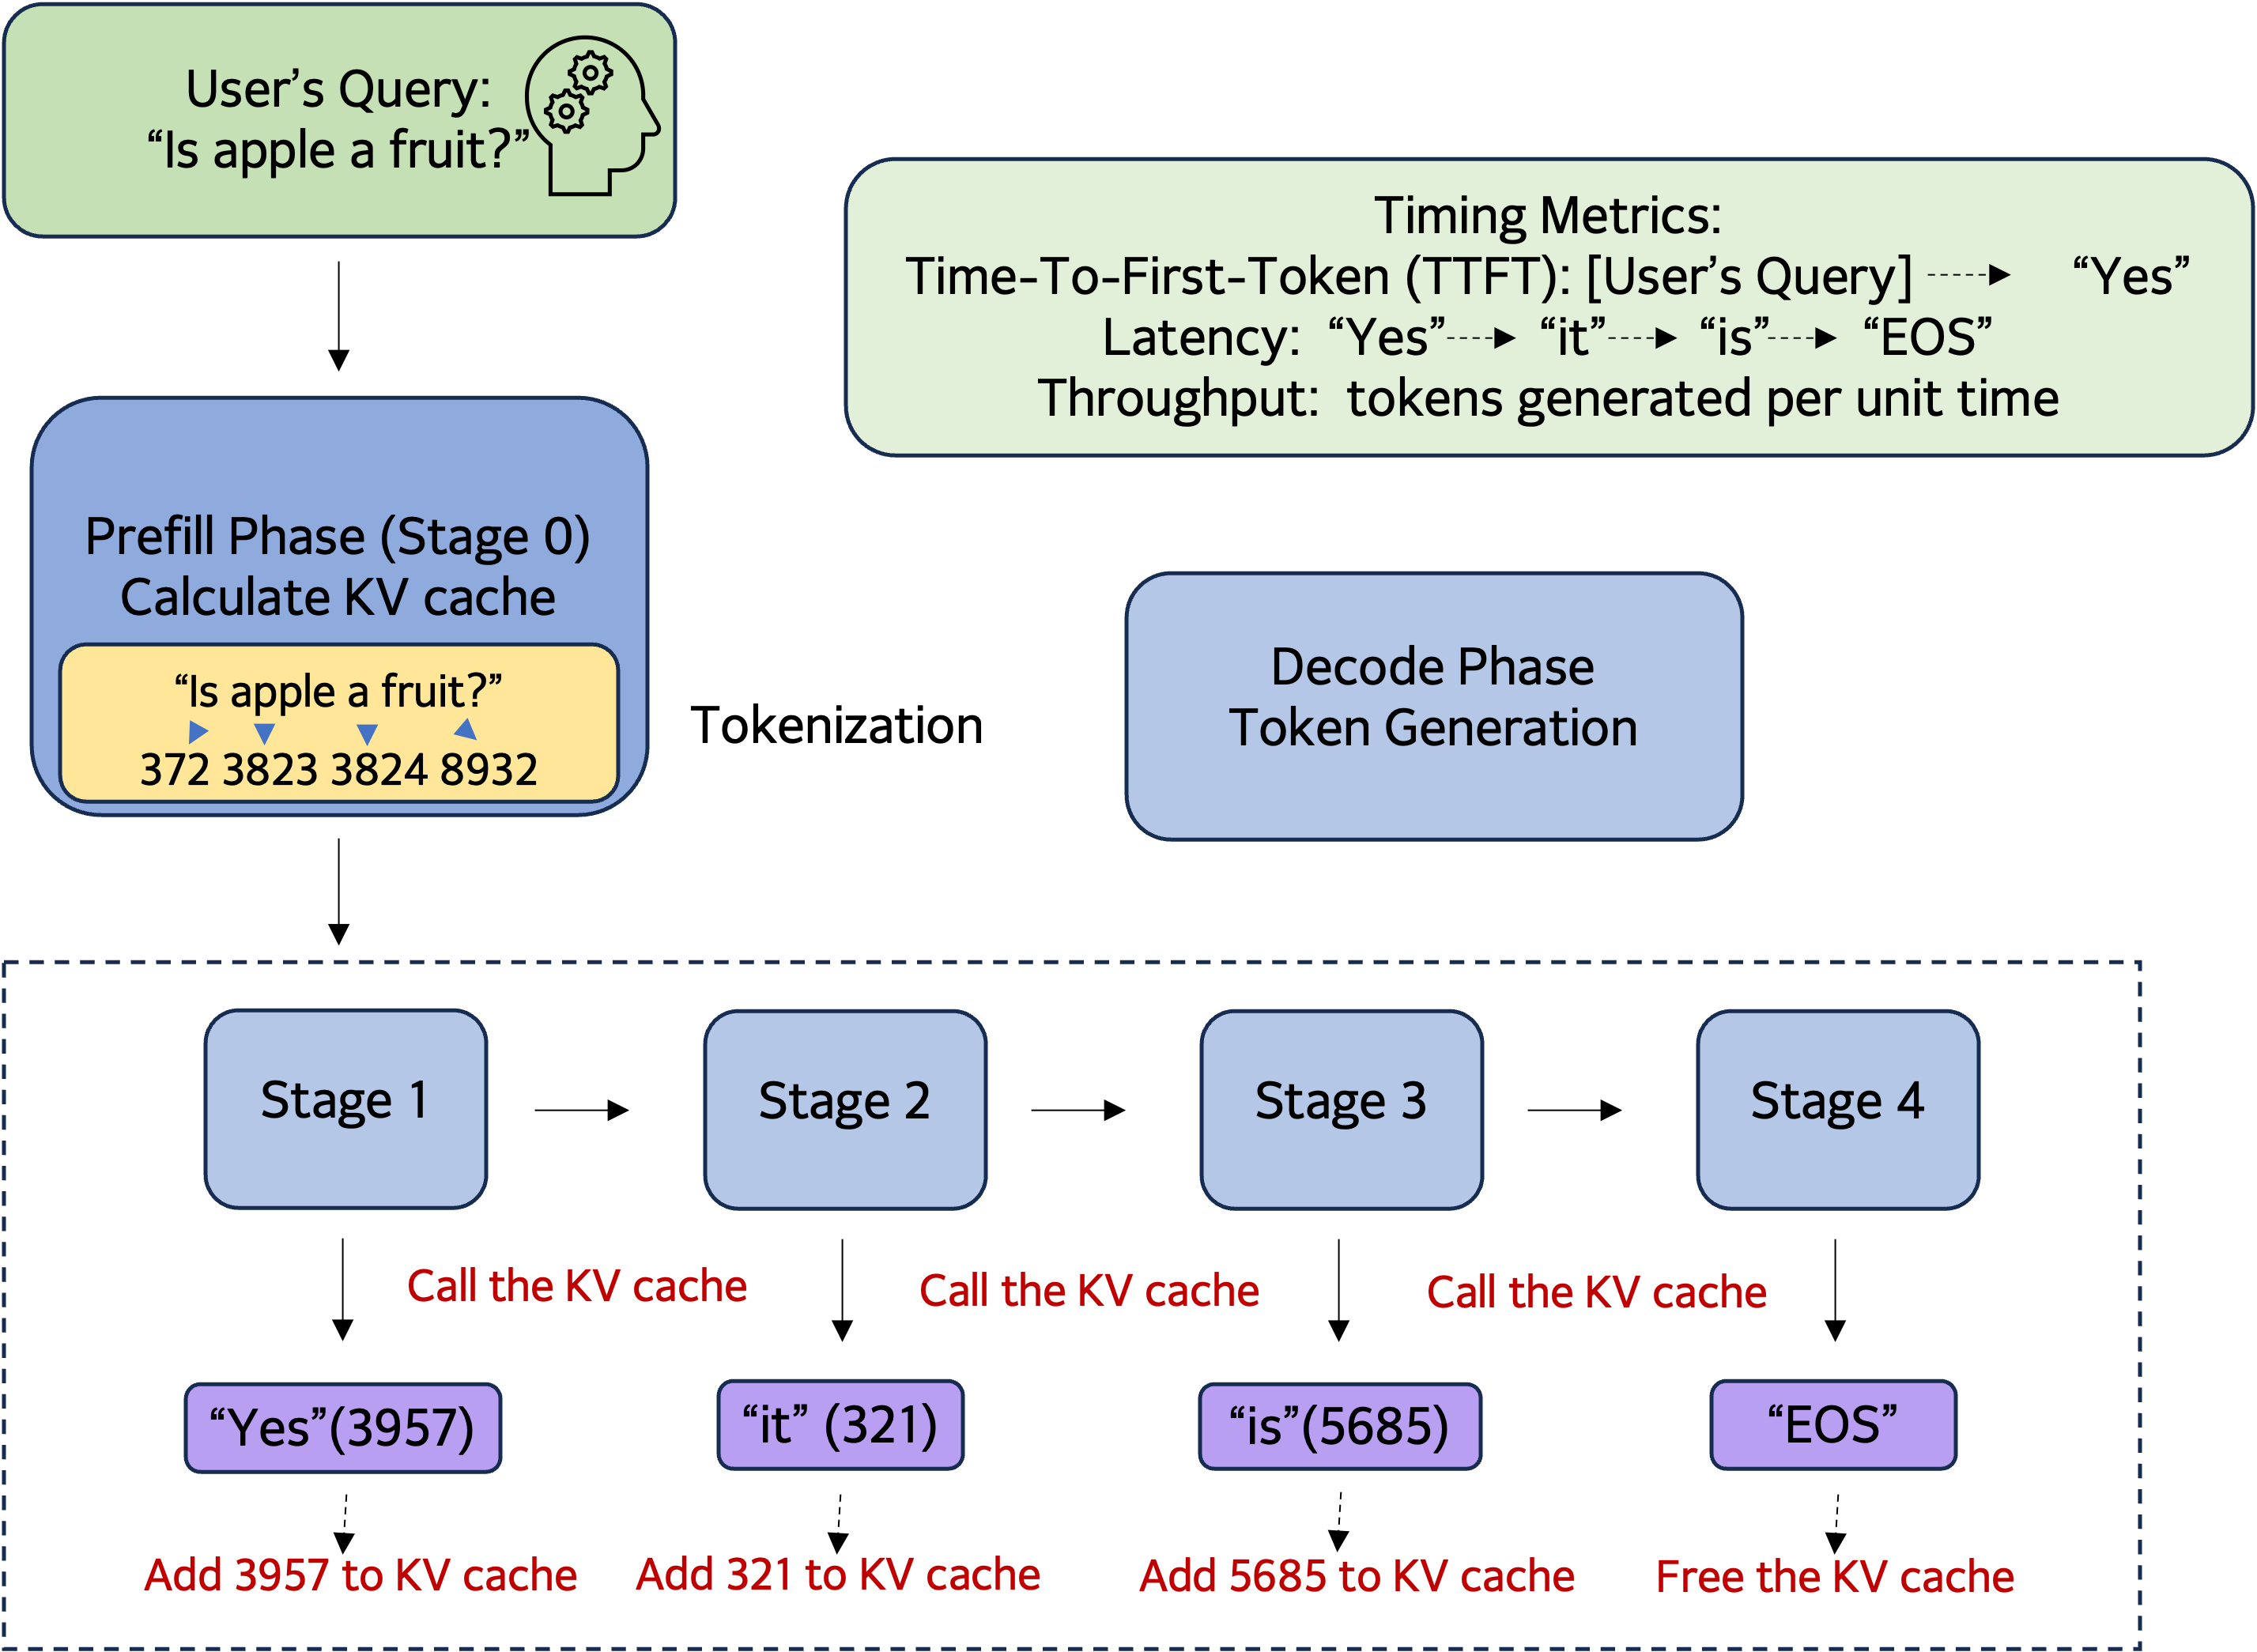
\includegraphics[width=0.8\linewidth]{fig_intro.png}
    \caption{An example of LLM inference.}
    \label{fig:intro_example}
\end{figure}

The inference workflow consists of two main phases. First, the \textbf{prefill step} processes the prompt to create the initial key-value (KV) cache.  
% For long prompts, like ``Tell me about the history of France,'' this step can use a lot of resources; splitting it into smaller parts (e.g., ``Tell me about'' and ``the history of France'') allows processing one part at a time to save memory.  
Next, the \textbf{decode step} builds the response one token at a time, updating the KV cache as it goes. This step increases memory use as the response gets longer. To make things more efficient, tasks can be grouped into \textbf{batches}, processing multiple prompts together. For example, a batch might include tokens from the prefill of a new prompt (e.g., ``What is the capital?'') and decode tasks from an ongoing response (e.g., ``How tall is Mount Everest?''), which needs careful handling of memory and computing power. Scheduling these batches well is very important for a few reasons. First, \textbf{memory limits} restrict how many tasks can run at once since the KV cache grows with each token; if memory runs out, data moves to slower storage, slowing things down. Second, scheduling must manage different goals: \textbf{Time to First Token (TTFT)}, the wait before the first token appears; \textbf{latency}, the time to finish the whole response; and \textbf{throughput}, the total rate of token creation. Keeping these balanced is key to a fast and efficient system. Third, \textbf{unpredictable prompt arrivals}---with different timing and complexity---make planning resources hard, so flexible approaches are needed.  
To handle this, systems can use smart scheduling methods. For instance, prioritizing short prompts can lower TTFT, while grouping similar tasks can boost throughput. Adjusting batch sizes based on available memory also helps avoid slowdowns. These strategies ensure the system stays responsive even when prompts vary or arrive unexpectedly.

Conventional scheduling methodologies, originally devised for domains like manufacturing or traditional computing, falter in this context due to the distinctive traits of LLM inference, notably its dynamic memory requirements and multi-phase pipeline. While recent engineering efforts have advanced system-level optimizations \citep{yu2022orca, kwon2023efficient, agrawal2023sarathi, pope2023efficiently,deepseekai2024deepseekv2strongeconomicalefficient,deepseekai2025deepseekv3technicalreport, sheng2023flexgen, patel2024splitwise, zhong2024distserve}, mathematical treatments remain scarce. A pioneering exception is \citet{jaillet2025onlineschedulingllminference}, which frames LLM inference as an online scheduling problem and develop algorithms with theoretic guarantee. However, different from our paper, it assumes perfect knowledge of the prompts' output lengths at arrival. Building on this, our work reconceptualizes the challenge as a multi-stage online scheduling problem with queueable requests under capacity limits. We propose an innovative approach integrating a fluid dynamics approximation to optimize steady-state performance and a \textbf{waiting for accumulated inference threshold (WAIT)} policy to manage stochastic arrivals, demonstrating near-optimal results in realistic scenarios without knowing the prompts' output in advance.

\subsection{Summary of Contributions}
In this work, we make the following contributions.
\paragraph*{Mathematical Model for Online Scheduling in LLM Inference}
We develop a multi-stage online scheduling model for LLM inference that incorporates queuable prompt under memory constraints (Section \ref{sec:model}). To approximate the system dynamics and establish a performance benchmark, we utilize a fluid approximation commonly employed in online resource allocation and queueing theory (Section \ref{sec:fluid}). 
% This approach is critical for optimizing resource use and ensuring efficient inference despite unpredictable prompt arrivals.

\paragraph*{Asymptotically Optimal Online Scheduling Algorithm}
In Section \ref{sec:wait}, we propose the \textit{Waiting for Accumulated Inference Threshold (WAIT)} algorithm for online scheduling in large language model (LLM) inference. As a warm-up, the algorithm is designed for cases where prompt output lengths are known. It sets processing thresholds based on prompt lengths and delays processing until these thresholds are reached. It utilizes the fluid approximation solution to enhance scheduling efficiency. We measure the algorithm's performance using the heavy-traffic limit from queueing theory and showing its asymptotic optimality. The proof is based on a novel analysis of waiting time dynamics through coupled random walks.

In Section \ref{sec:nested_wait}, we adapt the algorithm to more practical scenarios where prompt output lengths are unknown upon arrival, but their distributions are known. We introduce a \textit{nested WAIT} algorithm that divides prompts into segments based on their current output lengths, assigning distinct processing thresholds to each segment. Its asymptotic optimality is proven using a nested coupling technique.

\paragraph*{Experiments on Both Synthetic and Real Dataset Benchmarks.} In Section \ref{sec:experiments}, we evaluate our algorithm’s performance using synthetic prompt arrival flows and a real-world conversation dataset from \cite{zheng2023lmsys}.\footnote{The dataset is available at \url{https://huggingface.co/datasets/lmsys/lmsys-chat-1m}.} We compare our algorithm with benchmark scheduling methods vLLM in \cite{kwon2023efficient} and Sarathi in \cite{agrawal2023sarathi} running Llama2-7B on a single A100 GPU. Our algorithm outperforms both benchmarks in throughput and latency, demonstrating its effectiveness in practical LLM inference scenarios.

% The paper is structured to elucidate these advancements:
% \begin{itemize}
%     \item \textbf{Section 2} delineates the scheduling problem and its objectives.
%     \item \textbf{Section 3} details the fluid model for throughput optimization.
%     \item \textbf{Section 4} presents the booking-limit algorithm for known prompt types.
%     \item \textbf{Section 5} extends this to a nested algorithm for unknown output lengths.
%     \item \textbf{Section 6} reports numerical findings validating our approach.
%     \item \textbf{Section 7} concludes with implications and future research avenues.
% \end{itemize}

\subsection{Other Related Work}
\paragraph*{Online Scheduling Problem and Queueing System.} Classical online scheduling problems center on determining the optimal assignment of jobs that arrive sequentially, each requiring different completion times. In scenarios involving stochastic arrivals, foundational studies such as \cite{devanur2009adwords,vee2010optimal,cole2014sample,balkanski2016power,lattanzi2020online} have proposed algorithms that learn arrival patterns or distributions, iteratively refining their scheduling strategies. Beyond individual job processing, certain works have explored the integration of simultaneous batching and scheduling, grouping jobs into batches for improving efficiency (see, e.g., \cite{im2013online,lucier2013efficient,liu2015online,li2020online}). Additionally, online scheduling with queueable requests has been a significant focus within queueing theory. Fluid models, which serve as first-order approximations of stochastic systems, have been widely applied to design robust control strategies for queueing systems \cite{mandelbaum1998strong,maglaras2000discrete,bauerle2002optimal,liu2011network}. The heavy-traffic analysis further contributes by offering insights into the long-term behavior of these systems. However, these traditional heuristics in online scheduling and queueing systems fall short in addressing the dynamics of KV-cache and memory constraints encountered in LLM inference problems.

\paragraph*{LLM Inference.} Despite its critical engineering importance and widespread adoption, LLM inference lacks theoretical frameworks for analysis, with few studies addressing this gap. Instead, most research has concentrated on optimizing inference from a systems perspective. For instance, \cite{patel2023peeling} introduced "Splitwise" and \cite{zhong2024distserve} proposed "DistServe," both of which split the inference process into initial prompt handling and subsequent end-to-end pipeline execution. At the batching level, scheduling approaches such as those in \cite{yu2022orca}, \cite{agrawal2023sarathi}, and \cite{agrawal2024taming} focus on grouping requests to improve efficiency, a strategy that aligns closely with our own methodology. Additionally, \cite{deepseekai2024deepseekv2strongeconomicalefficient} leverages multi-head latent attention (MLA) with low-rank KV compression to enhance inference performance. More recent advancements include \cite{fu2025efficient}, which employs Kendall's Tau rule to prioritize prompts based on predicted output length, and \cite{jaillet2025onlineschedulingllminference}, which conducts a regret analysis of an algorithm with principle of prioritizing the shortest jobs first, demonstrating its near-optimal performance. However, \cite{jaillet2025onlineschedulingllminference} assumes perfect knowledge of arriving prompts' output lengths, while our Nested WAIT can provide theoretic guarantee even without this knowledge.


\subsection{Notations}
For integer $n\ge 1,$ we denote $[n]=\{1,2,\dots,n\}$ as the set of integers from $1$ to $n$. For $x\in\real$, denote $\lceil x\rceil$ as the smallest integer not smaller than $x$ and $\lfloor x\rfloor$ as the largest integer not greater than $x$. Denote $x_+=\max\{x, 0\}$. For set $S$, denote $|S|$ as its cardinality. For two functions $f(T)$ and $g(T)$, we use $f(T)=O(g(T))$ if there exists constant $c_1>0$ such that $f(T)\le c_1g(T)$ as $T\to+\infty$ and $f(T)=\Omega(g(T))$ if there exists constant $c_2>0$ such that $f(T)\ge c_2g(T)$ as $T\to +\infty$. 